%!TEX root = report.tex

\chapter{Travail Accompli}

\section{Introduction du chapitre}

Dans ce chapitre on procède à la présentation des cas utilisateur de
notre système ainsi que l'identification des acteurs impliqués dans ces
cas. Puis on décortique l’implémentation que nous proposons en citant
éventuellement nos motifs et intentions.

\section{Vue d'Ensemble}

\subsection{Identification des acteurs}

Notre système interagit essentiellement avec trois acteurs différents:

\begin{description}
\item[Le médecin] C'est l'acteur principal de notre système.

\item[Le service web] Source des données à acheminer vers le médecin.

\item[Système d'exploitation] Communique à notre système les
informations recueillies des divers composants qui nous intéressent
(localisation GPS/Network, état de la connectivité, état de la
batterie).

\end{description}

\subsection{Cas d'utilisations}

\begin{figure}
\center
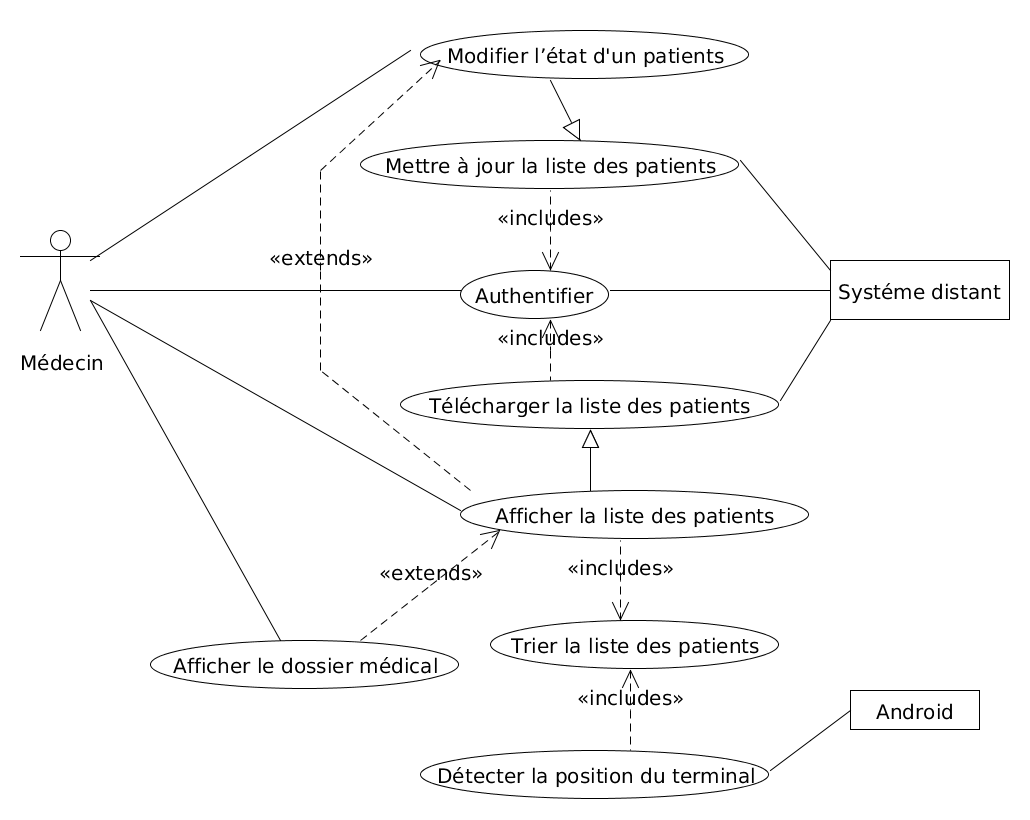
\includegraphics[width=0.8\textwidth]{diagrams/usecases}
\caption{Diagramme \gls{uml} des cas d'utilisation.}
\label{fig:usecase}
\end{figure}

\subsubsection{Cas: Authentifier}
\subsubsection{Cas: Notifier la proximité d'un patient}
\subsubsection{Cas: Détecter la position du terminal}
\subsubsection{Cas: Afficher la liste des patients}
\subsubsection{Cas: Télécharger la liste des patients}
\subsubsection{Cas: Modifier la liste des patients}
\subsubsection{Cas: Mettre à jour la liste des patients}

\subsection{Environnement de développement}%TODO
Plusieurs outils on était mise à contribution pour développer l'application, tant que sur le plan logiciel que matériel.

\subsubsection{Environnement Logiciel}
Voici une liste des outils logiciels utilisés pendant le développement de l'application.

\begin{description}

\item [Ubuntu 12.04] Système d'exploitation.\footnotemark[1]

\item [OpenJDK 6] \gls{jdk} version 6.\footnotemark[2]

\item [Eclipse Juno] Environnement de Développement Intégrer dans sa version \en{Service Release 2}.\footnotemark[3]

\item [\gls{adt} (plugin Eclipce)] Intégration des outils de développement fournit dans l'\gls{sdk} \android{}.\footnotemark[4]

\item [ObjectAid (plugin Eclipce)] Génération des diagrammes de classes.\footnotemark[5]

\item [PlantUML (plugin Eclipce)] Génération des diagrammes de séquences.\footnotemark[6]

\item [Git] Gestionnaire des versions\footnotemark[7].

\item [EGit (plugin Eclipse)] Intégration du gestionnaire de version.\footnotemark[8]

\item [Evolus Pencil] Génération de prototypes et des sketchs\footnotemark[9]
\end{description}

\footnotetext[1]{http://www.ubuntu.com}
\footnotetext[2]{http://openjdk.java.net}
\footnotetext[3]{http://www.eclipse.org}
\footnotetext[4]{https://developer.android.com/tools/sdk/eclipse-adt.html}
\footnotetext[5]{http://www.objectaid.com/}
\footnotetext[6]{http://plantuml.sourceforge.net/}
\footnotetext[7]{ttp://git-csm.com}
\footnotetext[8]{http://www.eclipse.org/egit/}
\footnotetext[9]{http://pencil.evolus.vn/}

\subsubsection{Environnement Matériel}
Le développement de l'application est fait avec une tablette Asus Nexus 7 (mise à jour à \android{} 4.2.2 \en{Jelly Bean}).



\section[Couche D'Accés aux Données]{Couche D'Accés aux Données}

Un des objectifs principales de ce projet étant de fournir une solution
d’accès aux données flexibles à fin de couvrir les besoins de chaque
client de manière individuelle. On a opté donc pour un modèle basé sur
l’implémentation de deux interfaces (figure \ref{fig:cls_dal}):

\begin{itemize}
\item Interface d'authentification.
\item Interface d’accès à la liste des patients.
\end{itemize}

\begin{figure}
\center
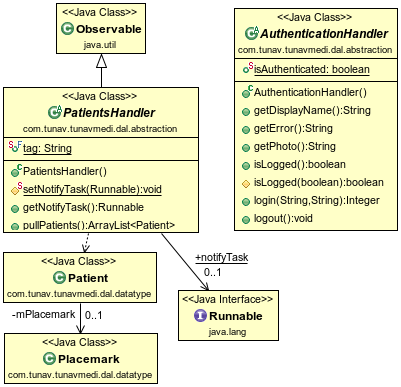
\includegraphics[totalheight=0.5\textheight]{diagrams/cls_dal}
\caption{Diagramme UML de classes des interfaces de la couche d’accès.}
\label{fig:cls_dal}
\end{figure}

L'idée est simple: pour chaque client, une implémentation spécifique à son infrastructure sera développée soit par son propre effectif, soit par une des équipes de \textsc{Tunav}, ou dans le cas idéal par une alliance formé par des agents des deux camps qui garantie une collaboration plus poussée pour des résultats meilleurs.
Ces ensembles d'interfaces nous permettent de construire notre application.

\subsection{Interface d'authentification}

\dev{com.tunav.tunavmedi.dal.abstraction.AuthenticationHandler} (figure
\ref{fig:cls_dal}) est une classe abstraite comportant les méthodes
requise par notre application pour effectué les actions
d'authentification, de dé-authentification, de vérification
d'authenticité ainsi l'obtention des informations associées à l'utilisateur
authentifier.

Malgré la variété des techniques d'authentification utilisée dans le domaine
informatique, l'étape d'acquisition des identificateurs de l'utilisateur
représente un point de départ commun. On utilise ce caractère dans l'interface
d'authentification en demandant à nos clients d'implémenter la méthode
\dev{login()} qui prend en argument l'identifiant et le mots de passe fourni par
le médecin, dans le cas d'une éventuelle erreur d'authentification,
l’implémentation met a notre disposition un message d'erreur accessible par la
méthode \dev{getError()}. Pour effectuer l’opération inverse le client
implémente la méthode \dev{logout()} supposée annoncer au service distant la dé-
authentification de l'utilisateur du terminal. Pour vérifier le l'état actuel de
la relation du terminal avec la base distante, on utilise le booléen retourné
par \dev{getStatus()}, utile dans les cas de déconnexion temporaire ou du
redémarrage de notre application. Les méthodes \dev{getDisplayName()} et
\dev{getPhoto()} retournent respectivement le nom de l'utilisateur et sa photo.

\subsection{Interface d’accès à la liste des patients}

\dev{com.tunav.tunavmedi.dal.abstraction.PatientsHandler} (figure
\ref{fig:cls_dal}) est une classe abstraite comportant les méthodes
requise par notre application pour effectué les actions de mise à jour de la liste des patients dans le deux sens (terminal $\rightarrow$ service et terminal $\leftarrow$ service), elle contient aussi un objet de type \dev{Runnable} associé au mécanisme de notification.

\subsubsection{Mécanisme de notification}

Le patron \textbf{Observateur} (\en{observer pattern}) (fig
\ref{fig:observer}) et un patron de conception couramment utilisé et qui
nous permet d'avoir une relation 1$\rightarrow$N entre divers objets. Le
patron observateur assume que l'objet qui contient les données est
séparé des l’objet qui les affiche et ces dites objets observe le
changement de ces données~\cite{jdp_observer}. Quant on implémente le
patron observateur, on réfère communément à l'objet contenant les
données par "Sujet"; et chacun des consommateurs des données par
"Observateur", Et chaque Observateurs implémente une interface préconçu
que le Sujet invoque quant les données changes~\cite{jdp_observer}.

\begin{figure}[H]
\center
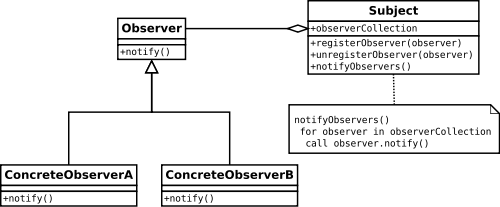
\includegraphics[width=0.8\textwidth]{Observer}
\caption{Diagramme UML du patron de conception Observateur~\cite{wiki:observer}}
\label{fig:observer}
\end{figure}

Dans le langage Java, ce patron est réalisé à travers la classe \dev{java.util.Observable} et l'interface \dev{Java.util.Observer}. Le Sujet hérite de la classe \dev{Observable} et les changements sont signalés par les méthodes \dev{setChanged()} et \dev{notifyObservers()} ou \dev{notifyObservers(Object message)}.

\subsubsection {Les objets de données}

\begin{figure}
\center
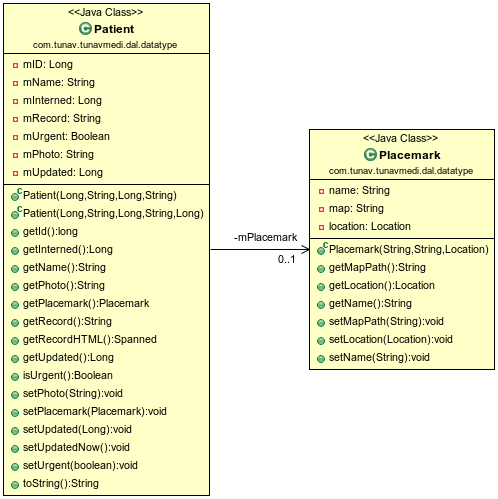
\includegraphics[width=0.8\textwidth]{diagrams/cls_dal_patient}
\caption{Diagramme UML de la classe \dev{Patient} }
\label{fig:cls_dal_patient}
\end{figure}

La communication des données avec le service distant se fait à travers l'objet \dev{com.tunav.tunavmedi.dal.datatype.Patient} (figure \ref{fig:cls_dal_patient}. Cet objet contient tous les informations requise pour la synchronisation et l'affichage et la gestion des patients, en particulier le dossier médical et la position actuelle du patient.

\paragraph{Synchronisation}
Étant sujet aux modifications de la part de l'application et du serveur distant, Un problème se pose pour savoir la version la plus à jour. Pour cela chaque modification apporté est suivi par une mise à jour de variable \dev{mUpdated} par le temps à cette instance précise (cette opération est interne à l'objet). En cas ou deux versions différentes de l'objet \dev{Patient} avec le même \dev{mID} et \dev{mUpdated}, le service est supposé favorisé sa version.

\paragraph{Dossier médical}

Le dossier médicale est fourni sous le format \en{HTML}. Cette représentation est idéal car elle nous permet de faire abstraction sur le format du dossier tel que sauvegarder par l'établissement client, la couche d’accès assurant éventuellement la conversion.


\paragraph{Position}

La position actuelle du patient est représenter par un objet \dev{Placemark}\footnote{com.tunav.tunavmedi.dal.datatype.Placemark} inspiré par la notation XML \gls{kml}. Les coordonnées sont représenter un objet de type \dev{Location}\footnote{android.location.Location}.

\subsection{Implémentation de tests}\label{subsection:dal_impl}

Le package \dev{com.tunav.tunavmedi.dal.sqlite} contiens une
implémentation de la couche d’accès abstraite (figure
\ref{fig:dal_sqlite}) réalisée dans le cadre de ce projet pour
pouvoir tester la solution. Cette implémentation est de caractère local
à l'application à travers les \gls{api} de la base de données
\dev{SQLite} qui fait parti de l'\gls{sdk} \android{}. En fait une
implémentation locale nous affranchie des problèmes qui peuvent se
produire dont la corrélation avec l'application est faible. Cette même
idée a influencé la mise en place même de cette implémentation qui à su
rester la plus simple possible en restant très proches des objets de
base de notre application.

\begin{figure}
\center
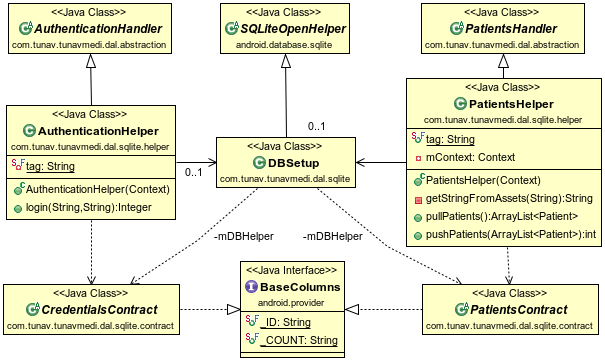
\includegraphics[angle=-90, width=0.8\textwidth]{diagrams/cls_dal_sqlite}
\caption{Diagramme de classe de l'implémentation de la couche d'accès de test à base de SQLite.}
\label{fig:dal_sqlite}
\end{figure}

Cette implémentation peut être subdivisée en trois éléments: Les \dev{Contrats}, les \dev{Helpers}, et la classe \dev{DBSetup}.

\paragraph{Les Contrats:}

Représente les contrats relative aux tables dans notre implémentation de
test. Chaque contrat implémente l'interface
\dev{BaseColumns}\footnote{android.provider.BaseColumns} et contient - entre autre - les
commandes SQL de création et de suppression de la dite table, des
éventuel index, et les commande d'insertion des données de test.

\paragraph{Les \en{Helpers}:} 

Ce sont les implémentations des classes abstraites qui définisse la
couche d’accès et présente les procédure d'extraction des données pré-
inséré dans nos table fictives en faisant appel à la classe
\dev{DBSetup} .

\paragraph[La classe \dev{DBSetup}:]{La classe \dev{DBSetup}:} 

Elle hérite de la classe \dev{SQLiteOpenHelper} et est destiner à
contrôler la création et l’accès à notre base de données de teste.



\section{Architecture Générale De L'Application}

L'application est subdivisé en deux parties majeurs représentés par deux classes de type \dev{android.app.Activity} :

\begin{description}

\item [LoginActivity] C'est une entité indépendante qui implémente la logique d'authentification, 

\item [MainActivity] C'est l'entité principale de notre solution mobile, elle relie les divers composants utilisés dans la transmission de la liste des patients, de la localisation et de la Conscience de l'état du terminal.

\end{description}

\subsection{LoginActivity}

%TODO

\begin{lstlisting}[language=xml, caption=Déclaration de LoginActivity dans AndroidManifest]

        <activity
            android:name="com.tunav.tunavmedi.activity.LoginActivity"
            android:label="@string/app_name"
            android:screenOrientation="portrait" >
            <intent-filter>
                <category android:name="android.intent.category.DEFAULT" />

                <action android:name="com.tunav.tunavmedi.action.LOGOUT" />
                <action android:name="com.tunav.tunavmedi.action.LOGIN" />
            </intent-filter>
        </activity>

\end{lstlisting}

\subsubsection[Diagrammes d'authentification]{Diagrammes \gls{uml} d'authentification}

\paragraph{Description textuelle}

\begin{description}

\item[Acteurs:] Docteur.

\item[Pré-condition:] Le docteur est déjà inscrit dans la base de données du service et son identifiant et mot de passe lui sont fournit.

\item[Scénario nominal:]

\begin{enumerate}

\item L'utilisateur lance ou retourne à l'application mobile donc \dev{MainActivity}.

\item \dev{MainActivity} détecte que l'utilisateur n'est pas déjà authentifier et actionne l'\gls{ui} d'authentification (appel à \dev{LoginActivity}).

\item L'utilisateur saisit son identifiant et mot de passe.

\item L'application interpelle le service pour vérifier que la combinaison identifiant / mot de passe est correcte.

\item Le service distant retourne une réponse favorable, \dev{LoginActivity} enregistre les données relative à l'utilisateur.

\item \dev{LoginActivity} invoque \dev{MainActivity}.

\end{enumerate}

\item [Enchaînement alternatif:]

\begin{itemize}

\item 2.a L'utilisateur est déjà authentifier:

\begin{enumerate}

\item La séquence d'authentification est sauter.

\end{enumerate}

\item 3.a L’identifiant et / ou le mot de passe comporte des erreurs (champs vide, mot de passe comporte moins des caractères que le minimum):

\begin{enumerate}

\item Affichage d'un message d'erreur.

\end{enumerate}

\item 5.a Le service distant retourne une réponse défavorable:

\begin{enumerate}

\item Le message d'erreur est extrait de l'interface d'authentification.

\item \dev{LoginActivity} affiche le message d'erreur.

\end{enumerate}

\end{itemize}

\end{description}

\paragraph{Diagramme de séquence}

Voir figure \ref{fig:seq_auth}

\begin{figure}
\center
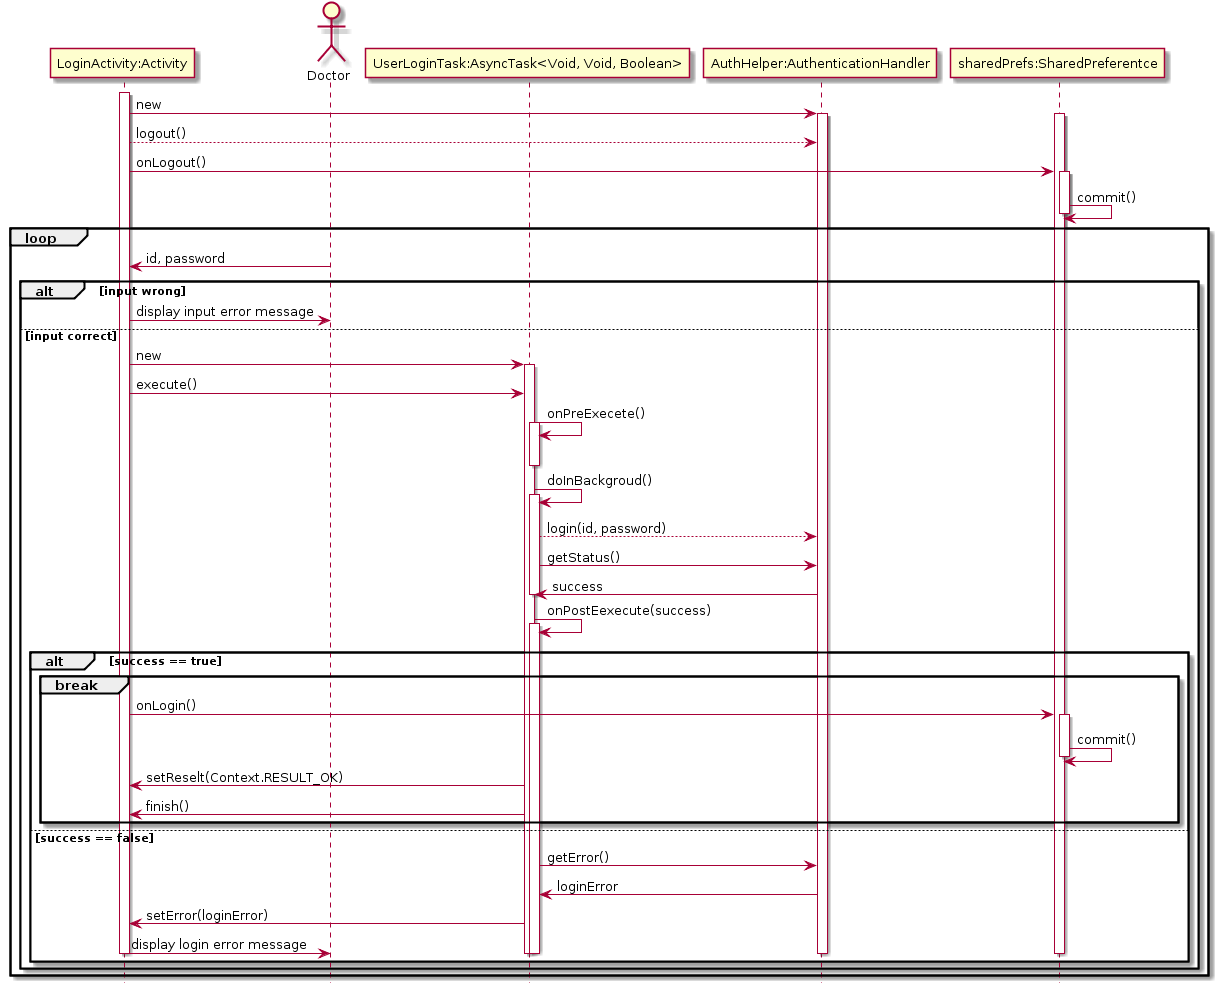
\includegraphics[angle=-90, width=\textwidth]{diagrams/seq_auth}
\caption{Diagramme \gls{uml} de séquence d'authentification.}
\label{fig:seq_auth}
\end{figure}



\subsection{MainActivity}

\begin{lstlisting}[language=xml, caption=Déclaration dans AndroidManifest de MainActivity]

        <activity
            android:name="com.tunav.tunavmedi.activity.MainActivity"
            android:label="@string/title_activity_main"
            android:screenOrientation="portrait" >
            <intent-filter>
                <action android:name="android.intent.action.MAIN" />

                <category android:name="android.intent.category.DEFAULT" />
                <category android:name="android.intent.category.LAUNCHER" />
            </intent-filter>
        </activity>

\end{lstlisting}

L'architecture globale du \dev{MainActivity}  (figure \ref{fig:cls_global})
est calquée sur Le patron "Vue Passive" (Passive View Pattern). Le patron
\en{Passive View} (fig \ref{fig:passive_view}) est une variation des
patrons \gls{mvc} et \gls{mvp}, de ce qui ce passe dans ces patrons.

L'interface utilisateur est divisée entre une Vue qui s'occupe de
l'affichage des données et un contrôleur qui répond aux interactions de
l'utilisateur. La différence majeur avec le \en{Passive View} est que la
Vue est complètement passive et n'ai pas responsable de sa mise à jour
depuis le modèle. Dans ce cas toute la logique de la Vue est dans le
contrôleur et aucune dépendance ni dans un sens au dans un autre entre
la Vue et le modèle~\cite{fowler:passive_view}.

\begin{figure}
\center
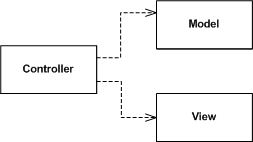
\includegraphics[width=0.6\textwidth]{passive_view}
\caption{Diagramme \gls{uml} de composant du patron \en{Passive Viev}~\cite{fowler:passive_view}}
\label{fig:passive_view}
\end{figure}

Ce patron est idéal dans notre cas pour deux raisons majeures:

\begin{itemize} 

\item Dans notre projet la Vue n'est pas la partie la plus importante
dans la mesure où l'objectif est d'intégrer un système développé
parallèlement, donc éventuellement avec une autre logique de
présentation. Déporter les interactions avec le modèle dans le
contrôleur permet d'intégrer d'autres implémentations d'affichage plus
facilement.

\item La nature même de cette procédure d’accès - à savoir l’aspect
abstrait, donc plus fragile - nous conduit à réduire les composants en
relations pour réduire la marge d'erreur possible et facilité les tests d’intégration.

\end{itemize}

\begin{figure}
\center
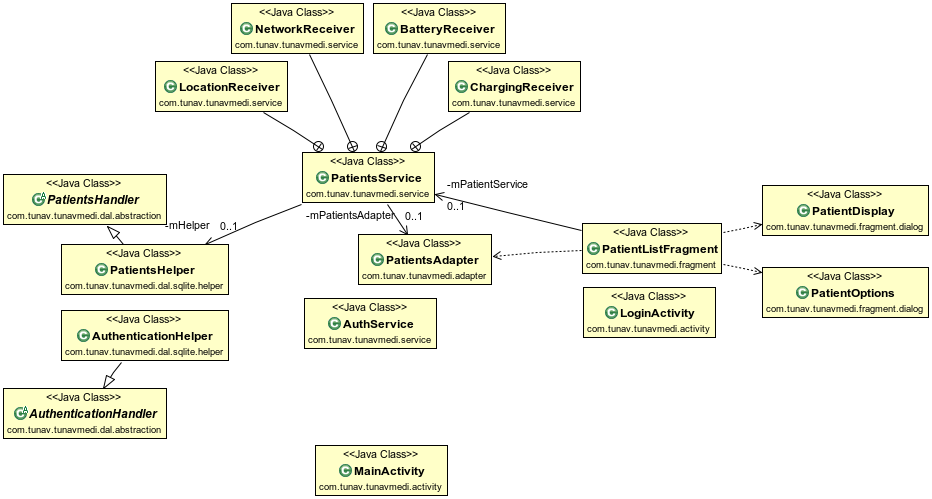
\includegraphics[angle=-90, width=0.9\textwidth]{diagrams/cls_global}
\caption{Diagramme de classes \gls{uml} de l'architecture générale de l'application.}
\label{fig:cls_global}
\end{figure}

Dans la suite de ce chapitre, on procède à l'explication détaillée du Contrôleur
et de la Vue, pour le Modèle veuillez vous reporter au point
\ref{subsection:dal_impl}.

\subsubsection{Le Contrôleur}

\begin{figure}
\center
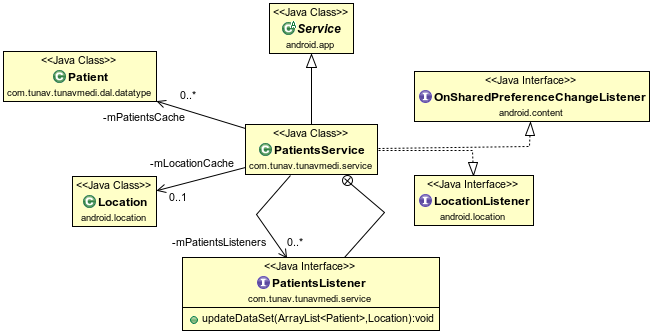
\includegraphics[width=0.8\textwidth]{diagrams/cls_ctrl}
\caption{Diagramme \gls{uml} de classe du contrôleur.}
\label{fig:cls_ctrl}
\end{figure}

\begin{lstlisting}[language=xml, caption=Déclaration dans AndroidManifest du PatientService]

        <service
            android:name="com.tunav.tunavmedi.service.PatientsService"
            android:exported="false" >
            <intent-filter>
                <category android:name="android.intent.category.DEFAULT" />
            </intent-filter>
        </service>

\end{lstlisting}

Notre contrôleur est matérialisé par l'objet
\dev{PatientService}\footnote{com.tunav.tunavmedi.service.PatientService} qui
hérite de la classe \dev{Service}\footnote{android.app.Service}. L'\gls{api}
\android{} définie un service comme étant un composant de l'application qui
représente soit la volonté de cette application de faire des longs opérations
sans d’interagir avec l'utilisateur ou d’offrir des fonctionnalités à
l'intention des autres applications\cite{api:service}.

\paragraph{Localisation}
Pour la localisation, le contrôleur implémente les techniques présenter dans \ref{sss:android_localisation}
%TODO

\paragraph{Conscience de l'état du terminal}

Le tableau \ref{tab:status} représente la configuration que le contrôleur suit dans le cas d'un changement d’état du terminal. En particulier l'inutilité de cherché la position actuelle du terminal dans le cas ou celui ci est en charge, encore en cas ou le terminal annonce que la batterie est faible on procède à un mode d’économie d’énergie pour évité entre autre la corruption des données.

\begin{table}[H]
\centering
\begin{tabular}{|c|c|c|}
\hline
&\textsf{Mises à jour} & \textsf{Localisation}\\
\hline
\textsf{Batterie Faible} & déactivé & déactivé\\
\hline
\textsf{Batterie en Charge} & activé & déactivé\\
\hline
\textsf{Pas de connectivité} & déactivé & activé\\
\hline
\end{tabular}
\caption{Configuration du contrôleur en réponse au changement d’état du terminal}
\label{tab:status}
\end{table}

\subparagraph{Connectivité}

Les permissions cités dans le listing \ref{lst:permission_network} sont nécessaire pour s’abonnées aux événement liée a la connectivité du terminal. Le \dev{NetworkReceiver}\footnote{com.tunav.tunavmedi.broadcastreceiver.NetworkReceiver} (listing \ref{lst:receiver_network}) s'occupe de notifier les intéressés, dans notre cas le contrôleur, via des \dev{SharedPreferences}.

\begin{lstlisting}[language=xml, label=lst:permission_network, caption=Déclaration dans AndroidManifest des permission d’accès à l’état des interfaces réseaux.]

<uses-permission android:name="android.permission.ACCESS_NETWORK_STATE" />

\end{lstlisting}

\begin{lstlisting}[language=xml, label=lst:receiver_network, caption=Déclaration dans AndroidManifest du  NetworkReceiver]

        <receiver
            android:name="com.tunav.tunavmedi.broadcastreceiver.NetworkReceiver"
            android:enabled="true" >
            <intent-filter>
                <action android:name="ConnectivityManager.CONNECTIVITY_ACTION" />
            </intent-filter>
        </receiver>

\end{lstlisting}

\subparagraph{Batterie}

Le \dev{BatteryReceiver}\footnote{com.tunav.tunavmedi.broadcastreceiver.BatteryReceiver} (listing \ref{lst:receiver_battery}) fait savoir au contrôleur via des \dev{SharedPreferences} si la batterie est faible ou pas.

\begin{lstlisting}[language=xml, label=lst:receiver_battery, caption=Déclaration dans AndroidManifest du BatteryReceiver.]

        <receiver
            android:name="com.tunav.tunavmedi.broadcastreceiver.BatteryReceiver"
            android:enabled="true" >
            <intent-filter>
                <action android:name="android.intent.action.BATTERY_LOW" />
                <action android:name="android.intent.action.BATTERY_OK" />
            </intent-filter>
        </receiver>

\end{lstlisting}

\subparagraph{Mobilité}
Le \dev{ChargingReceiver}\footnote{com.tunav.tunavmedi.broadcastreceiver.ChargingReceiver} (listing \ref{lst:receiver_network}) est destiné à notifier le contrôleur quant le terminal est connecté ou déconnecter du  chargeur via des \dev{SharedPreferences}.

\begin{lstlisting}[language=xml, label=lst:receiver_charging, caption=Déclaration dans AndroidManifest ChargingReceivers.]

        <receiver
            android:name="com.tunav.tunavmedi.broadcastreceiver.ChargingReceiver"
            android:enabled="true" >
            <intent-filter>
                <action android:name="android.intent.action.ACTION_POWER_CONNECTED" />
                <action android:name="android.intent.action.ACTION_POWER_DISCONNECTED" />
            </intent-filter>
        </receiver>

\end{lstlisting}

\subsubsection{La Vue}

\begin{figure}
\center
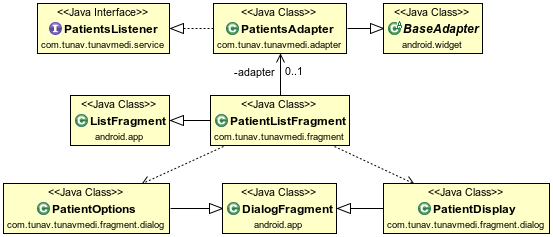
\includegraphics[width=0.8\textwidth]{diagrams/cls_view}
\end{figure}

Le système d'exploitation \android{} rend facile le développement des applications qui tourne sur des appareils qui possèdes des formes et des tailles d’écran différents, une des améliorations apporter dans \android{} 3.0 Honeycomb sont les \dev{Fragment} censé décomposé les fonctionnalité et les interfaces utilisateur d'une l'application \android{} en des modules réutilisables. Notre implémentation de la Vue prend avantage de cet introduction en utilisant des \dev{Fragment} et ce de se compose essentiellement de 4 composants:

\begin{description}

\item[PatientAdapter] Représente un \dev{BaseAdapter} qui joue le rôle d'un adaptateur entre la \dev{PatientListFragment} et notre contrôleur, la communication avec celui-ci est assuré à travers l'interface \dev{PatientsListener}.

\item[PatientListFragment] Hérite de l'objet \dev{PatientListFragment} et s'occupe de l'affichage de la liste des patients.

\item[PatientDisplay] Un \dev{DialogFragment} qui s'occupe de l'affichage du dossier médicale du patient

\item[PatientOptions] Un \dev{DialogFragment} qui permet au docteur de modifier la condition d'un patient.

\end{description}

\paragraph{Algorithme de Trie}

L'or de l'affichage de la liste des patients, une opération de trie est appliquée pour facilité la tache du docteur en mettant en valeur les cas qui requière le plus son attention.
L’algorithme se base sur les conditions suivantes (dans l'ordre):

\begin{enumerate}

\item Le patient est un cas urgent ou non.

\item Le patient est à proximité ou non.

\item La date d'admission du patient.

\end{enumerate}

Cette opération est réalisé la méthode static \dev{java.util.Collections.sort()} en utilisant notre propre objet de type \dev{java.util.Comparator<Patient>} qui respecte les conditions citées ci-dessus.


\paragraph{Affichage du dossier médicale}

Le dossier étant sous la forme d'un document HTML, pour l'afficher on utilise un \dev{android.webkit.WebView} (voir listing \ref{lst:xml_patientdisplay})qui nous offre les capacités d'un vrais navigateur web.


\begin{lstlisting}[language=xml, label=lst:xml_patientdisplay, caption=Déclaration XML du \gls{ui} utilisé par PatientDisplay]

<?xml version="1.0" encoding="utf-8"?>
<RelativeLayout xmlns:android="http://schemas.android.com/apk/res/android"
    android:id="@+id/task_dialog"
    style="@style/ListFrontContent"
    android:layout_width="wrap_content"
    android:layout_height="wrap_content" >

    <ImageView
        android:id="@+id/task_dialog_image"
        style="@style/ListImage" />

    <TextView
        android:id="@+id/task_dialog_title"
        style="@style/ListTitle"
        android:layout_width="match_parent"
        android:layout_height="wrap_content"
        android:layout_toRightOf="@id/task_dialog_image"
        android:maxLines="2"
        android:textIsSelectable="false" />

    <TextView
        android:id="@+id/task_dialog_timer"
        style="@style/ListDescription"
        android:layout_width="wrap_content"
        android:layout_height="wrap_content"
        android:layout_alignBottom="@id/task_dialog_image"
        android:layout_alignParentRight="true"
        android:maxLines="1"
        android:textIsSelectable="false" />

    <View
        android:id="@+id/task_dialog_separator"
        android:layout_width="fill_parent"
        android:layout_height="1dp"
        android:layout_below="@id/task_dialog_image"
        android:layout_margin="5dp"
        android:background="@android:color/darker_gray" />

    <WebView
        android:id="@+id/task_dialog_description"
        style="@style/ListDescription"
        android:layout_width="match_parent"
        android:layout_height="wrap_content"
        android:layout_below="@id/task_dialog_separator"
        android:textIsSelectable="true" 
        android:singleLine="false"/>

</RelativeLayout>

\end{lstlisting}


\section{Déploiement et Tests}

\subsection{Détecteur de bugs: Android Lint}

\begin{figure}[H]
\center
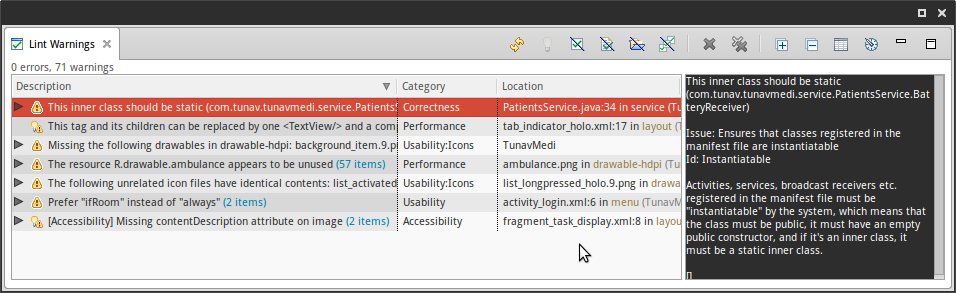
\includegraphics[width=0.9\textwidth]{lint}
\caption{Problèmes potentiels dans notre application détectés par Android Lint.}
\label{fig:lint}
\end{figure}

\android{} \en{Lint} (figure \ref{fig:lint}) est un outil introduit dans la version 16 de \gls{adt} qui scanne les code sources des projets \android{} afin d'y détecter des mal-fonctions potentiels.

Quelques exemples de types d'erreurs que cet outil permet de détecter sont:

\begin{itemize}

\item Translations manquantes ou inutilisés.

\item Les problèmes de performance dans les \dev{Layout}.

\item Ressources inutilisées

\item Tableau de taille inconsistante (dans le cas ou le tableau est défini dans des configurations différentes).

\item Problème d'accessibilités et d'internationalisation.

\item Problème d'icônes (Tailles manquantes, doubles, fausse résolution).

\item Problème d'usabilité .

\item Erreurs dans le \dev{Manifest}.

\end{itemize}

Dans Eclipse, \android{} Lint est disponible à travers le menu Window $\rightarrow$ Show View $\rightarrow$ Other... puis on sélectionne \en{Lint Warning} dans la fenêtre qui s'affiche (figure \ref{fig:lint_eclipse}).

\begin{figure}
\center
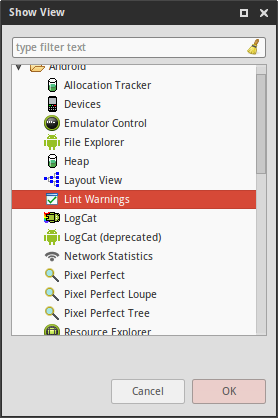
\includegraphics[width=0.4\textwidth]{lint_eclipse}
\caption{Accéder à Android Lint dans Eclipse}
\label{fig:lint_eclipse}
\end{figure}

\section{Conclusion du chapitre}